% notes
\providecommand{\redo}[1]{{\color{red} #1}}
\providecommand{\rebuttal}[1]{{#1}}


\providecommand{\nbc}[3]{
 {\colorbox{#3}{\bfseries\sffamily\scriptsize\textcolor{white}{#1}}}
 {\textcolor{#3}{\sf\small\textit{#2}}}
 }
\definecolor{annotcolo}{rgb}{0.1,0.1,0.9}
\providecommand{\nj}[1]{\nbc{NJ}{#1}{annotcolo}}


% config
\providecommand{\smalltextsc}[1]{\textsc{\small #1}}
\providecommand{\scripttextsc}[1]{\textsc{\scriptsize #1}}
\providecommand{\tinytextsc}[1]{\textsc{\tiny #1}}

% sysnames
\providecommand{\livecodebench}{\smalltextsc{LiveCodeBench}}
\providecommand{\lcb}{\smalltextsc{LCB}}
\providecommand{\livecodebenchtitle}{\textsc{LiveCodeBench}}


% general
\providecommand{\llm}{\smalltextsc{LLM}\xspace}
\providecommand{\llms}{\smalltextsc{LLMs}\xspace}
\providecommand{\chainot}{\smalltextsc{COT}\xspace}
\providecommand{\python}{\smalltextsc{Python}\xspace}




%models

%openai
\providecommand{\openai}{\smalltextsc{OpenAI}}
\providecommand{\gpts}{\smalltextsc{GPTs}\xspace}
\providecommand{\codedavinci}{\smalltextsc{Code-Davinci-002}\xspace}
\providecommand{\gptthreefiveturbo}{\smalltextsc{GPT-3.5-turbo}\xspace}
\providecommand{\gptfour}{\smalltextsc{GPT-4}\xspace}
\providecommand{\gptfourturbo}{\smalltextsc{GPT-4-Turbo}\xspace}
\providecommand{\gptfouro}{\smalltextsc{GPT-4-O}\xspace}

%deepmind
\providecommand{\alphacode}{\smalltextsc{AlphaCode}\xspace}
\providecommand{\alphacodeB}[1]{\smalltextsc{AlphaCode-#1B}\xspace}

%anthropic
\providecommand{\claude}{\smalltextsc{Claude}\xspace}
\providecommand{\claudes}{\smalltextsc{Claudes}\xspace}
\providecommand{\claudetwo}{\smalltextsc{Claude-2}\xspace}
\providecommand{\claudethrees}{\smalltextsc{Claude-3s}\xspace}
\providecommand{\claudeinstantone}{\smalltextsc{Claude-Ins-1}\xspace}
\providecommand{\claudeopus}{\smalltextsc{Claude-3-Opus}\xspace}
\providecommand{\claudesonnet}{\smalltextsc{Claude-3-Sonnet}\xspace}

%google
\providecommand{\gemini}{\smalltextsc{Gemini}\xspace}
\providecommand{\geminis}{\smalltextsc{Geminis}\xspace}
\providecommand{\geminipro}{\smalltextsc{Gemini-Pro}\xspace}
\providecommand{\geminiproonefive}{\smalltextsc{Gemini-Pro-1.5}\xspace}
\providecommand{\geminiflash}{\smalltextsc{Gemini-Flash}\xspace}
\providecommand{\geminiultra}{\smalltextsc{Gemini-Ultra}\xspace}

%meta 
\providecommand{\cllamas}{\smalltextsc{CodeLLaMas}\xspace}
\providecommand{\cllama}{\smalltextsc{CodeLLaMa}\xspace}
\providecommand{\cllamains}{\smalltextsc{CodeLLaMa-Ins}\xspace}
\providecommand{\cllamabase}{\smalltextsc{CodeLLaMa-Base}\xspace}
\providecommand{\cllamaB}[1]{\smalltextsc{CL-Ins-#1B}\xspace}
\providecommand{\cllamacommonB}[1]{CL-#1B}
\providecommand{\cllamabaseB}[1]{\smalltextsc{CL-Base-#1B}\xspace}
\providecommand{\cllamaBList}{\smalltextsc{CL-Ins-\{7, 13, 34\}B}\xspace}
\providecommand{\cllamabaseBList}{\smalltextsc{CL-Base-\{7, 13, 34\}B}\xspace}

\providecommand{\llamas}{\smalltextsc{LLaMa-3s}\xspace}

\providecommand{\llamabase}{\smalltextsc{L3-Base}}
\providecommand{\llamabaselist}{\smalltextsc{L3-Base-\{7, 70\}B}\xspace}
\providecommand{\llamainslist}{\smalltextsc{L3-Ins-\{7, 70\}B}\xspace}
\providecommand{\llamaB}[1]{\smalltextsc{L3-Ins-#1B}\xspace}
\providecommand{\llamabaseB}[1]{\smalltextsc{L3-Base-#1B}\xspace}

%finetunes
\providecommand{\wizardlong}{\smalltextsc{WizardCoder}\xspace}
\providecommand{\wizard}{\smalltextsc{WC-34B}\xspace}
\providecommand{\wizardtwo}{\smalltextsc{WC-33B}\xspace}
\providecommand{\phind}{\smalltextsc{Phind-34B}\xspace}
\providecommand{\magicoders}{\smalltextsc{MagiCoders}\xspace}
\providecommand{\magicoder}[1]{\smalltextsc{MC-#1B}\xspace}
\providecommand{\magicoderBLit}{\smalltextsc{MC-\{6.7, 7\}B}\xspace}

%deepseek
\providecommand{\deepseek}{\smalltextsc{DeepSeek}\xspace}
\providecommand{\deepseekbase}{\smalltextsc{DeepSeek-Base}\xspace}
\providecommand{\deepseekinstruct}{\smalltextsc{DeepSeek-Instruct}\xspace}
\providecommand{\deepseeks}{\smalltextsc{DeepSeeks}\xspace}
\providecommand{\deepseekcode}[1]{\smalltextsc{DS}-#1B\xspace}
\providecommand{\deepseekcodeins}{\smalltextsc{DS-Ins}\xspace}
\providecommand{\deepseekcodeB}[1]{\smalltextsc{DS-Ins-#1B}\xspace}
\providecommand{\deepseekbaseB}[1]{\smalltextsc{DS-Base-#1B}\xspace}
\providecommand{\deepseekcodeBList}{\smalltextsc{DS-Ins-\{1.3, 6.7, 33\}B}\xspace}
\providecommand{\deepseekcodebaseBList}{\smalltextsc{DS-Base-\{1.3, 6.7, 33\}B}\xspace}

% codeqwen
\providecommand{\codeqwen}{\smalltextsc{CodeQwen}\xspace}
\providecommand{\codeqwenchat}{\smalltextsc{CodeQwen-Chat}\xspace}

%mistral

\providecommand{\mixtral}{\smalltextsc{Mixtral}\xspace}
\providecommand{\codestral}{\smalltextsc{Codestral}\xspace}
\providecommand{\mistrallarge}{\smalltextsc{Mistral-L}\xspace}
\providecommand{\mistral}{\smalltextsc{Mistral}\xspace}

% bigcode

\providecommand{\starcoder}{\smalltextsc{StarCoder}\xspace}
\providecommand{\starcodertwo}{\smalltextsc{StarCoder2}\xspace}
\providecommand{\starcodertwobase}{\smalltextsc{StarCoder2-Base}\xspace}
\providecommand{\sctwoinsB}[1]{\smalltextsc{SC2-#1B}\xspace}
\providecommand{\sctwobaseB}[1]{\smalltextsc{SC2-Base-#1B}\xspace}
\providecommand{\sctwobaseBList}{\smalltextsc{SC2-Base-\{3,7,15\}B}\xspace}

% cohere
\providecommand{\commandr}{\smalltextsc{CMD-R}\xspace}
\providecommand{\commandrplus}{\smalltextsc{CMD-R+}\xspace}


% datasets
\providecommand{\thestack}{\smalltextsc{Stack}\xspace}
\providecommand{\apps}{\smalltextsc{APPS}\xspace}
\providecommand{\contests}{\smalltextsc{Code-Contests}\xspace}
\providecommand{\humaneval}{\smalltextsc{HumanEval}}
\providecommand{\humanevalplus}{\smalltextsc{HumanEval+}}
\providecommand{\mbpp}{\smalltextsc{MBPP}}
\providecommand{\cruxeval}{\smalltextsc{CRUXEval}}
\providecommand{\codet}{\smalltextsc{CodeT}}
\providecommand{\xcode}{\smalltextsc{xCodeEval}\xspace}
\providecommand{\codescope}{\smalltextsc{CodeScope}\xspace}
\providecommand{\taco}{\smalltextsc{TACO}\xspace}
\providecommand{\usacobench}{\smalltextsc{USCAOBench}\xspace}
%coding websites
\providecommand{\leetcode}{\smalltextsc{LeetCode}\xspace}
\providecommand{\atcoder}{\smalltextsc{AtCoder}\xspace}
\providecommand{\codeforces}{\smalltextsc{CodeForces}\xspace}
\providecommand{\html}{\smalltextsc{HTML}\xspace}

\providecommand{\easy}{\smalltextsc{Easy}\xspace}
\providecommand{\medium}{\smalltextsc{Medium}\xspace}
\providecommand{\hard}{\smalltextsc{Hard}\xspace}

%website scrapes
\providecommand{\problem}{\smalltextsc{$P$}\xspace}
\providecommand{\solution}{\smalltextsc{$S$}\xspace}
\providecommand{\tests}{\smalltextsc{$T$}\xspace}
\providecommand{\testspublic}{\smalltextsc{$T_{p}$}\xspace}
\providecommand{\testshidden}{\smalltextsc{$T_{h}$}\xspace}
\providecommand{\contestdate}{\smalltextsc{$D$}\xspace}

% metrics
\providecommand{\passmetric}[1]{\smalltextsc{Pass@}#1\xspace}



% %%%%
\lstset{
  basicstyle=\ttfamily\small,
  columns=fullflexible,
  % frame=single,
  breaklines=true,
  postbreak=\mbox{$\hookrightarrow$\space},
  rulecolor=\color{black},
}
\definecolor{codegreen}{rgb}{0,0.6,0}
\lstdefinestyle{mystyle}{  
    commentstyle=\color{codegreen},
    keywordstyle=\color{blue},
    basicstyle=\ttfamily\small,
    breakatwhitespace=false,        
    breaklines=true,                 
    captionpos=b,                    
    keepspaces=true,                 
    showspaces=false,                
    showstringspaces=false,
    showtabs=false,                  
    tabsize=2
}
\lstset{style=mystyle}

% if you use cleveref..

% %%%%%%%%%%%%%%%%%%%%%%%%%%%%%%%%
% % THEOREMS
% %%%%%%%%%%%%%%%%%%%%%%%%%%%%%%%%
% \theoremstyle{plain}
% \newtheorem{theorem}{Theorem}[section]
% \newtheorem{proposition}[theorem]{Proposition}
% \newtheorem{lemma}[theorem]{Lemma}
% \newtheorem{corollary}[theorem]{Corollary}
% \theoremstyle{definition}
% \newtheorem{definition}[theorem]{Definition}
% \newtheorem{assumption}[theorem]{Assumption}
% \theoremstyle{remark}
% \newtheorem{remark}[theorem]{Remark}

% % Todonotes is useful during development; simply uncomment the next line
% %    and comment out the line below the next line to turn off comments

% \input{math_commands.tex}
% \newcommand{\todo}[1]{\textcolor{red}{[TODO: #1]}}
\newcommand{\term}[1]{\emph{#1}}
\definecolor{rewriteblue}{RGB}{0,70,170}
\definecolor{mygreen}{RGB}{226,240,217}
\definecolor{myblue}{RGB}{222,235,247}
\definecolor{myorange}{RGB}{251,229,214}
\definecolor{lightblue}{RGB}{232,242,255}
\definecolor{lightorange}{RGB}{255,241,224}
\definecolor{good}{HTML}{1B7837}
\definecolor{bad}{HTML}{B2182B}
\newcommand{\needsrewrite}[1]{\textcolor{rewriteblue}{[SOURCE-DERIVED; REWRITE: #1]}}
\newenvironment{rewriteblock}{%
  \par\begingroup\color{rewriteblue}%
  \noindent
}{%
  \par\endgroup
}
\newenvironment{draftblock}{%
  \par\noindent
}{%
  \par
}
\newcommand{\sourcepaper}[2]{}

\definecolor{lightgreen}{HTML}{C4FFCF}
\definecolor{codegreen}{rgb}{0,0.6,0}

\newcommand{\red}[1]{\textbf{\textcolor{red}{#1}}}
\newcommand{\green}[1]{\textbf{\textcolor{ForestGreen}{#1}}}
\newcommand{\cmark}{\ding{51}}
\newcommand{\xmark}{\ding{55}}
\newcommand{\benchmark}{\textsc{CRUXEval}\xspace}
\newcommand{\benchmarki}{\textsc{CRUXEval-I}\xspace}
\newcommand{\benchmarko}{\textsc{CRUXEval-O}\xspace}
\newcommand{\codellamamed}{\textsc{Code Llama 13B}\xspace}
\newcommand{\codellamalarge}{\textsc{Code Llama 34B}\xspace}
\providecommand{\multirow}[3]{#3}
\providecommand{\hdashline}[1][]{\midrule}
\NewDocumentCommand{\cdashline}{m o}{}
\providecommand{\makecell}[1]{\begin{tabular}{@{}c@{}}#1\end{tabular}}
\providecommand{\smallsec}[1]{\textbf{#1\,\,}}
\providecommand{\llm}{\textsc{LLM}\xspace}
\providecommand{\llms}{\textsc{LLMs}\xspace}
\providecommand{\lean}{\textsc{Lean}\xspace}
\providecommand{\setstretch}[1]{}
\providecommand{\smallsim}{\mathrel{\sim}}
\providecommand{\subfloat}[2][]{%
  \begin{minipage}{0.49\textwidth}%
  \centering
  #2%
  \if\relax\detokenize{#1}\relax\else\subcaption{#1}\fi
  \end{minipage}%
}

\DeclareMathOperator*{\argmax}{arg\,max}
\DeclareMathOperator*{\argmin}{arg\,min}
\lstdefinelanguage{Lean}{
  morekeywords={theorem,lemma,def,by,have,show,calc,let,fun,match,with,if,then,else,import,open,namespace,end,where,structure,inductive,example},
  sensitive=true,
  morecomment=[l]{--},
  morecomment=[s]{/-}{-/},
  morestring=[b]"
}
\lstdefinelanguage{triton}{
  morekeywords={tl,triton,jit,program_id,load,store,arange,zeros,where,constexpr,block_ptr,dtype},
  sensitive=true,
  morecomment=[l]{\#},
  morestring=[b]"
}
\lstdefinelanguage{CUDA}{
  morekeywords={__global__,__device__,__shared__,__constant__,__host__,__syncthreads,threadIdx,blockIdx,blockDim,gridDim},
  sensitive=true,
  morecomment=[l]{//},
  morecomment=[s]{/*}{*/},
  morestring=[b]",
  morestring=[b]'
}
\lstdefinelanguage{Rust}{
  morekeywords={as,break,const,continue,crate,else,enum,extern,false,fn,for,if,impl,in,let,loop,match,mod,move,mut,pub,ref,return,self,Self,static,struct,super,trait,true,type,unsafe,use,where,while,async,await,dyn},
  sensitive=true,
  morecomment=[l]{//},
  morecomment=[s]{/*}{*/},
  morestring=[b]",
  morestring=[b]'
}
\lstdefinelanguage{Python}{
  morekeywords={and,as,assert,break,class,continue,def,del,elif,else,except,False,finally,for,from,global,if,import,in,is,lambda,None,nonlocal,not,or,pass,raise,return,True,try,while,with,yield},
  sensitive=true,
  morecomment=[l]{\#},
  morecomment=[s]{\"\"\"}{\"\"\"},
  morecomment=[s]{\'\'\'}{\'\'\'},
  morestring=[b]',
  morestring=[b]"
}
\lstdefinelanguage{json}{
  morekeywords={true,false,null},
  sensitive=false,
  morestring=[b]",
  morecomment=[l]{//},
}

\lstdefinestyle{mystyle}{
  commentstyle=\color{codegreen},
  keywordstyle=\color{blue},
  basicstyle=\ttfamily\footnotesize,
  breakatwhitespace=false,
  breaklines=true,
  captionpos=b,
  keepspaces=true,
  showspaces=false,
  showstringspaces=false,
  showtabs=false,
  tabsize=2
}
\lstdefinestyle{boxed}{
  frame=single,
  breaklines=true,
  postbreak=\mbox{$\hookrightarrow$\space},
  commentstyle=\color{codegreen},
  keywordstyle=\color{blue},
  basicstyle=\ttfamily\footnotesize,
  breakatwhitespace=false,
  captionpos=t,
  keepspaces=true,
  showspaces=false,
  showstringspaces=false,
  showtabs=false,
  tabsize=2
}
\lstdefinestyle{specblock}{
  frame=single,
  breaklines=true,
  basicstyle=\ttfamily\scriptsize,
  keepspaces=true,
  showstringspaces=false,
  columns=fullflexible
}
\DefineVerbatimEnvironment{codebox}{Verbatim}{fontsize=\small}
\DefineVerbatimEnvironment{examplecodebox}{Verbatim}{fontsize=\small}
\lstdefinestyle{reasoning}{
  breaklines=true,
  commentstyle=\color{codegreen},
  keywordstyle=\color{blue},
  breakautoindent=0pt,
  breakindent=0pt,
  basicstyle=\itshape\footnotesize,
  breakatwhitespace=true,
  captionpos=t,
  keepspaces=true,
  showspaces=false,
  showstringspaces=false,
  showtabs=false
}
\lstdefinestyle{mystylesmaller}{
  commentstyle=\color{codegreen},
  keywordstyle=\color{blue},
  basicstyle=\ttfamily\scriptsize,
  breaklines=true,
  captionpos=b,
  keepspaces=true,
  showspaces=false,
  showstringspaces=false,
  showtabs=false,
  tabsize=2
}
\lstdefinestyle{mystyletiny}{
  commentstyle=\color{codegreen},
  keywordstyle=\color{blue},
  basicstyle=\ttfamily\tiny,
  breaklines=true,
  captionpos=b,
  keepspaces=true,
  showspaces=false,
  showstringspaces=false,
  showtabs=false,
  tabsize=2
}
\lstdefinestyle{leancompact}{
  language=Lean,
  basicstyle=\fontsize{3}{3.5}\ttfamily,
  breaklines=true,
  captionpos=b,
  keepspaces=true,
  showspaces=false,
  showstringspaces=false,
  showtabs=false,
  frame=none
}
\lstset{
  style=mystyle,
  columns=fullflexible,
  frame=single,
  postbreak=\mbox{$\hookrightarrow$\space},
  rulecolor=\color{black},
  moredelim=[is][\color{red}]{!*}{*!},
  literate={₀}{{$_0$}}1
           {₁}{{$_1$}}1
           {₂}{{$_2$}}1
           {₃}{{$_3$}}1
           {₄}{{$_4$}}1
           {₅}{{$_5$}}1
           {₆}{{$_6$}}1
           {₇}{{$_7$}}1
           {₈}{{$_8$}}1
           {₉}{{$_9$}}1
           {¹}{{$^1$}}1
           {²}{{$^2$}}1
           {³}{{$^3$}}1
           {⁻}{{$^-$}}1
           {·}{{$\cdot$}}1
           {×}{{$\times$}}1
           {∀}{{$\forall$}}1
           {∃}{{$\exists$}}1
           {ℕ}{{$\mathbb{N}$}}1
           {ℚ}{{$\mathbb{Q}$}}1
           {ℝ}{{$\mathbb{R}$}}1
           {ℤ}{{$\mathbb{Z}$}}1
           {∧}{{$\wedge$}}1
           {∨}{{$\vee$}}1
           {∈}{{$\in$}}1
           {∉}{{$\notin$}}1
           {∑}{{$\sum$}}1
           {∫}{{$\int$}}1
           {∣}{{$\mid$}}1
           {≠}{{$\ne$}}1
           {≡}{{$\equiv$}}1
           {≤}{{$\le$}}1
           {≥}{{$\ge$}}1
           {←}{{$\leftarrow$}}1
           {→}{{$\to$}}1
           {↑}{{$\uparrow$}}1
           {⊢}{{$\vdash$}}1
           {⟨}{{$\langle$}}1
           {⟩}{{$\rangle$}}1
           {…}{{\ldots}}1
}

\makeatletter
\def\@captype{lstlisting}
\lst@AddToHook{Init}{\def\@captype{lstlisting}}
\makeatother

\theoremstyle{plain}
\newtheorem{theorem}{Theorem}[chapter]
\newtheorem{lemma}[theorem]{Lemma}
\newtheorem{proposition}[theorem]{Proposition}
\newtheorem{corollary}[theorem]{Corollary}

\theoremstyle{definition}
\newtheorem{definition}[theorem]{Definition}
\newtheorem{example}[theorem]{Example}

\theoremstyle{remark}
\newtheorem{remark}[theorem]{Remark}



\providecommand{\smallsim}{\smallsym{\mathrel}{\sim}}

\makeatletter
\providecommand{\smallsym}[2]{#1{\mathpalette\make@small@sym{#2}}}
\providecommand{\make@small@sym}[2]{%
  \vcenter{\hbox{$\m@th\downgrade@style#1#2$}}%
}
\providecommand{\downgrade@style}[1]{%
  \ifx#1\displaystyle\scriptstyle\else
    \ifx#1\textstyle\scriptstyle\else
      \scriptscriptstyle
  \fi\fi
}
\makeatother


\subsection[Overfitting to HumanEval+]{Overfitting to HumanEval+}

We first compare the code generation performance of models on \humanevalplus{} vs. \livecodebench{},
shown in Figure~\ref{fig:he_vs_lcb}. We observe two distinct clusters of models, shown in red and green. The green cluster shows models that perform 
similarly on both benchmarks, consisting mostly of base and closed-access models. 
The red cluster shows models that perform significantly better on \humanevalplus{} than \livecodebench{}. Careful analysis reveals that
this cluster consists primarily of fine-tuned variants of open-access models, strongly indicative of overfitting
or data contamination.  In particular, we draw attention to \deepseekcodeB{1.3}, which achieves
$60\%$ on \humanevalplus{} but only $26\%$ on \lcb{}-Easy.
These results mirror what we found with \benchmark{} in Section~\ref{sec:cruxeval-beyond-score}: a class of
models with a high HumanEval (\humanevalplus{} in this case) score with no corresponding gains
on a different benchmark.

Overall, the lesson is that high scores on familiar benchmarks can be ambiguous.
Sometimes, it may indicate general programming abilities, but other times it may be due to benchmark-specific adaptation. 
It is crucial to compare across a varied suite of different benchmarks to understand the full picture, and we should be 
careful of techniques that promote overfitting rather than developing general abilities.

\begin{figure}[!t]
    \centering
    \includegraphics[width=0.99\textwidth]{figures/main_results/lcb_vs_he.png}
  \vspace{-3pt}
    \caption{
        Scatter plot comparing \passmetric{1} of models on \humanevalplus{} versus \lcb{}-Easy{} (time-window Sep $2023$ to May $2024$).
        The green-shaded region marks models with aligned performance across benchmarks, while the red-shaded region marks models with much stronger performance on \humanevalplus{}.
    }

        \label{fig:he_vs_lcb}
        \vspace{-15pt}
\end{figure}


\subsection{Role of Post-Training}
Next, we analyze the performance of base models vs. post-trained models. In terms of 
base models, we see that \llamabase{} and \deepseek{} significantly outperform \cllama{} and
\starcodertwo. However, these differences may partially be due to the training data
distribution. For example, \starcodertwo uses competition coding problems in its
pre-training corpus.

Our benchmark also shows that post-training significantly improves performance, as 
\llamaB{70}, \deepseekcodeB{33}, and \phind{} achieve 28.3, 23.6, and 21.0 \passmetric{1} on \lcb{},
improving over their base models by 8.2, 7.3, and 9.5 points respectively.

On the other hand, while base models generally fall into the green cluster of models,
post-trained models generally end up in the red cluster.  
We hypothesize that compared to data used in closed-access models, the fine-tuning 
datasets for open models are lacking in diversity and quality, which may lead to poorer
generalization. 

\subsection{Gap Between Closed and Open Models}

In Figure~\ref{fig:lcb-beyond-open-closed-gap}, we investigate the gap between
open-access and closed-access models. 
We already started to see this Section~\ref{sec:cruxeval-beyond-score}, where we found that GPT-4 had already 
distinguished itself at CRUXEval compared to other models. It showed good performance on both CRUXEval and HumanEval seemingly
without overfitting to either, and benefited significantly more from chain-of-thought than 
any other models. 
Overall, on \livecodebench{}, closed models generally outperform open models.
However, the gap is not uniform, as models like \llamaB{70}, \mixtral{}, and \deepseekcodeB{33}
perform on-par with the weaker closed models like \geminipro{} and \gptthreefiveturbo{}, and 
\claudesonnet. However, this varies across scenarios, as closed-access models perform better in the 
test output prediction and code execution scenarios. This suggests that strong base models
and high-quality post-training data can partially close the gap, but that there are several
capabilities where closed models still have a significant lead. 


\begin{figure}[H]
  \centering
  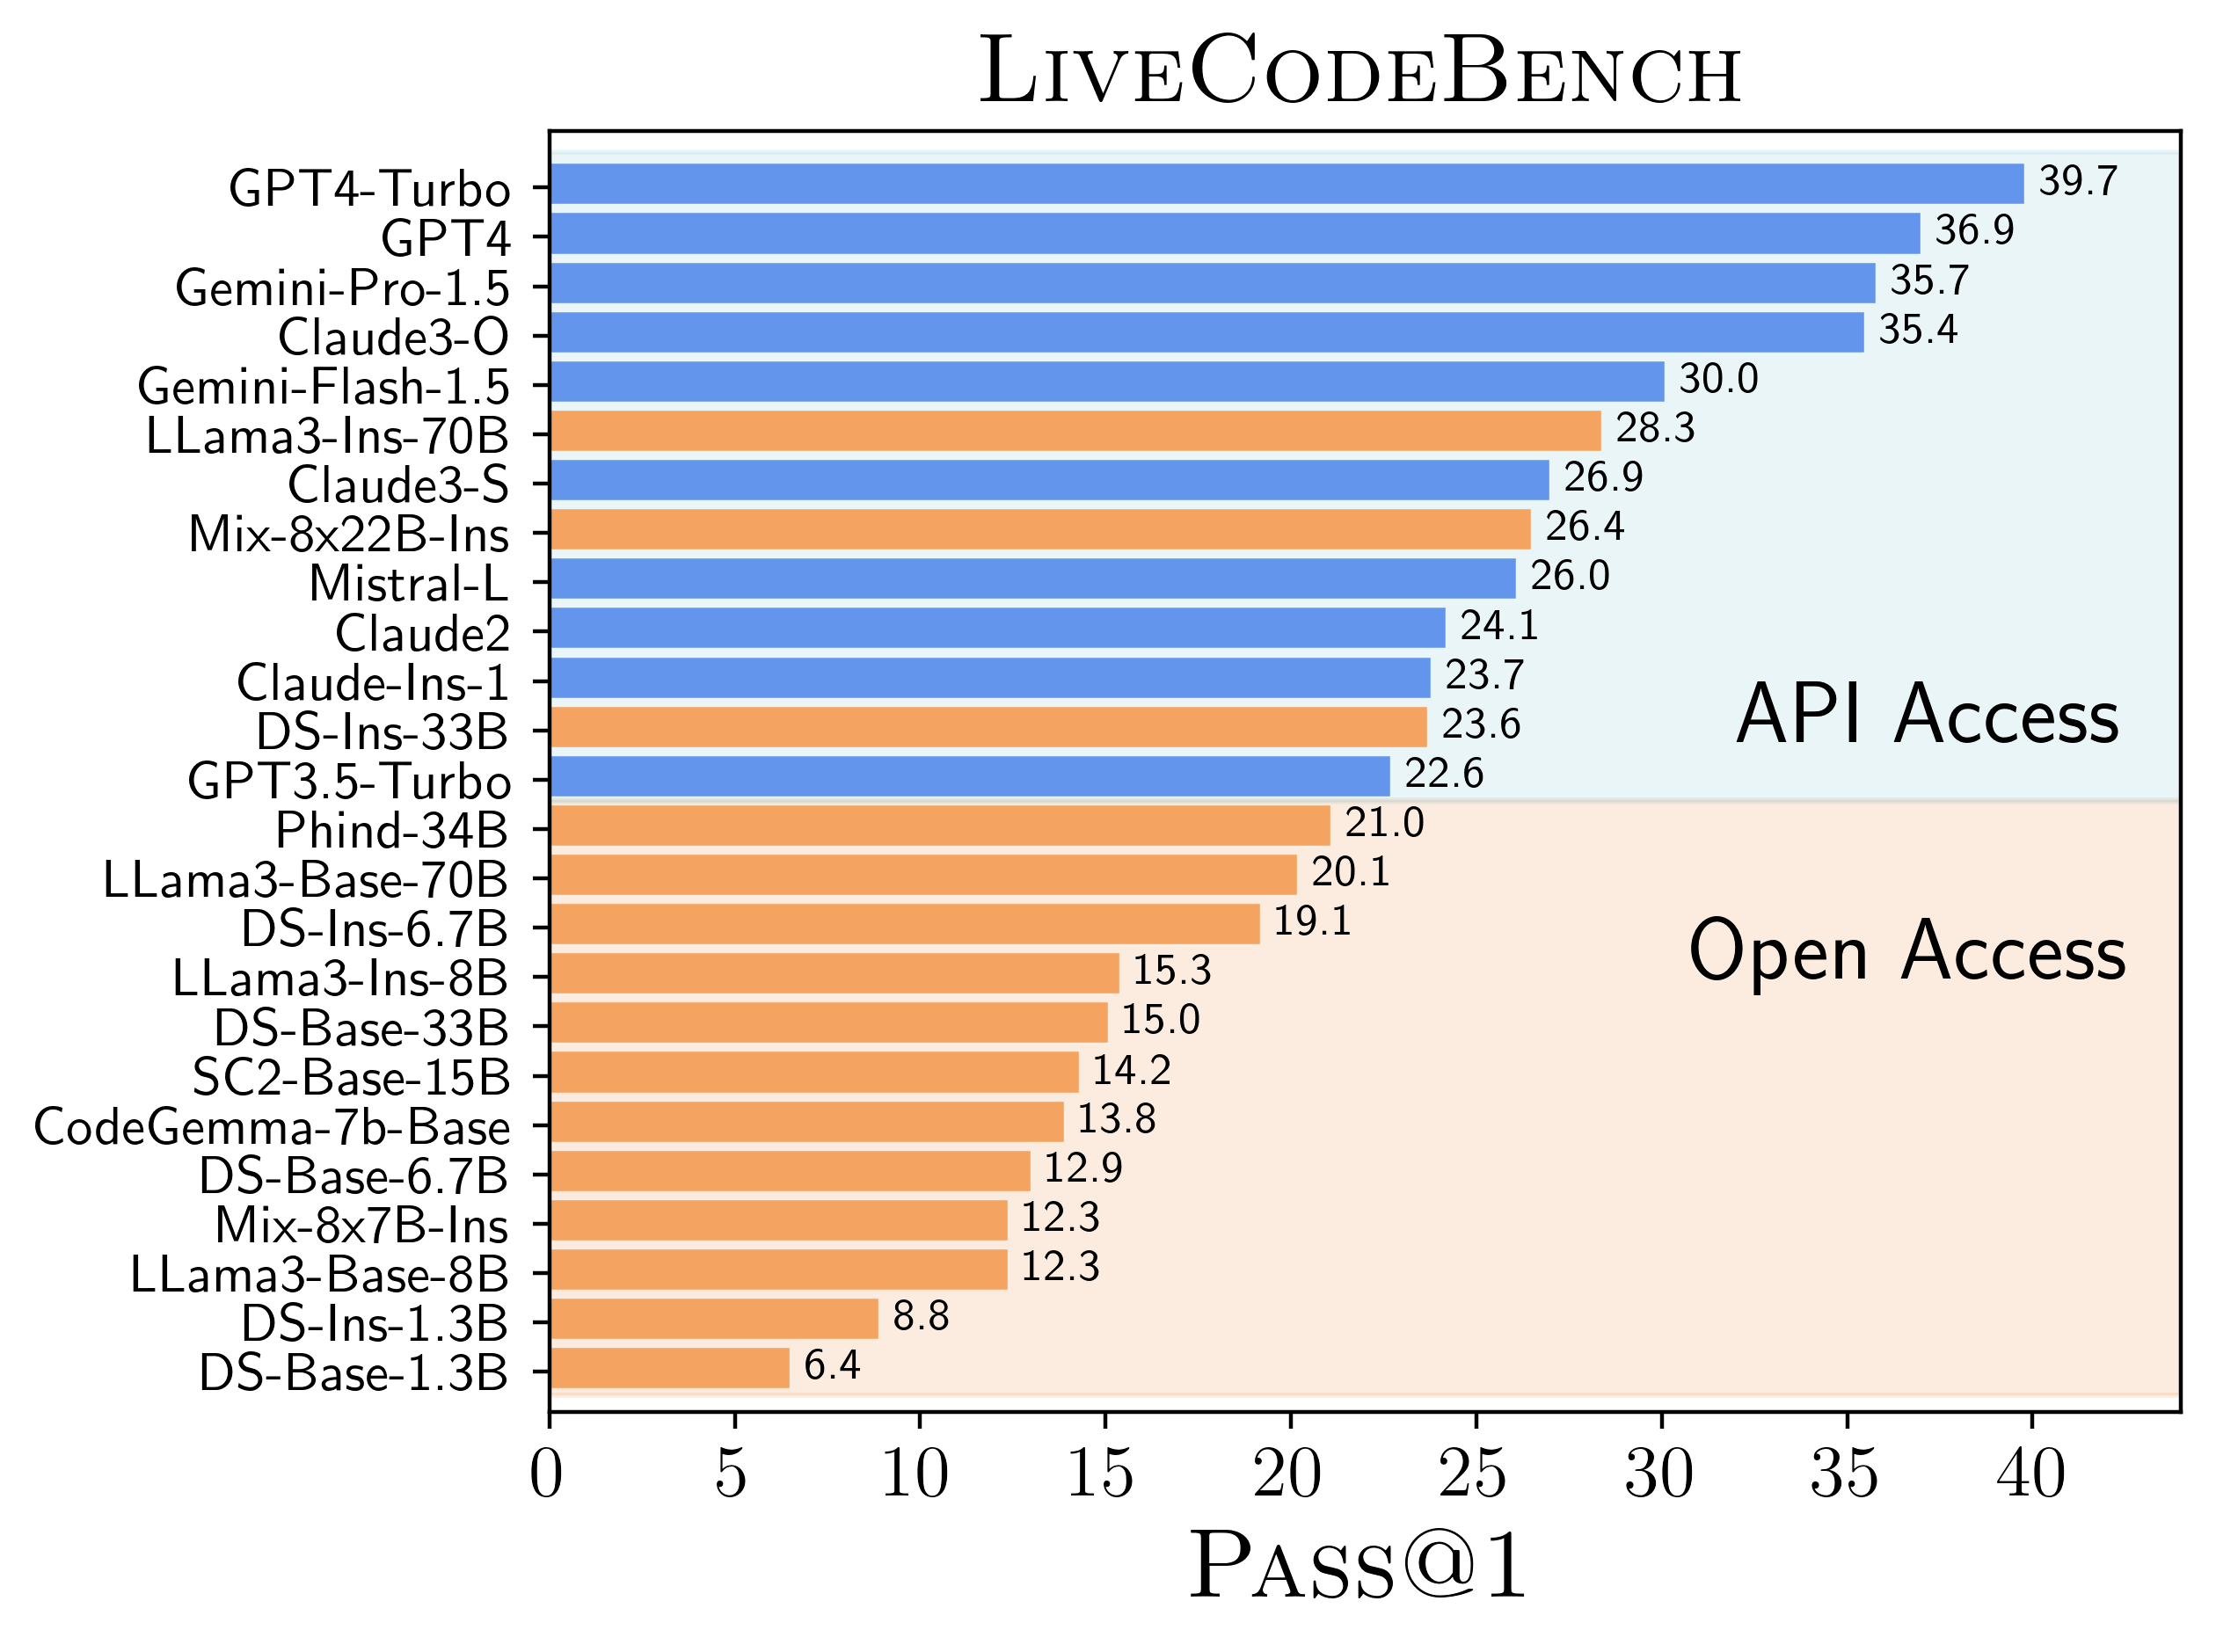
\includegraphics[width=0.65\linewidth]{figures/overview/lc_barchart.png}
  \caption{Comparison of open-access and closed-access models on the
  \livecodebench{}-Easy code-generation scenario.}
  \label{fig:lcb-beyond-open-closed-gap}
\end{figure}
